\section{Experimental Evaluation}
\label{sec:evaluation}

\subsection{Questions, Workloads, and Measurement}
% P:E1
We first measure complete service cost and trace the differences to candidate access. Fixed-catalog studies then isolate response maintenance, followed by independent checks of decision evidence. Table~\ref{tab:evidence_scope} identifies the input populations, measurement policies, and completion counts.

% P:E2
The main domain uses the full Bitcoin Alpha and OTC projections~\cite{snapalpha,snapotc,kumar2016edge}. They have $n=3{,}783$ and $5{,}881$ vertices and logical catalogs of $M=7{,}140{,}884$ and $17{,}271{,}859$ candidates. Directed ratings are aggregated into undirected signed weighted pairs; zero aggregates and self-links are removed. The resulting natural half-integer edge weights are preserved. Every root nonedge admits a positive insertion of weight $1/16$, and every negative root edge admits a magnitude-preserving flip.

% P:E2a
Three synthetic opinion workloads exercise gradual changes, independent uniform opinions, and graph-correlated opinions produced by signed-neighbor averaging, all quantized to $2^{-16}$. Each request starts at the structural root with empty Grams and no answer cache, uses $\delta=0$, and allows at most 15 commits. This setup measures response reuse within edit trajectories. Q1 and Q4 contain one and four opinion requests, respectively, with structural preparation charged once.

% P:E3
All paths share endpoint screens, responses, transfer, equality resolution, and acceptance rules. D materializes the catalog and root-cap index. S scans blocks of 65,536 rows. H emits row-frontier batches of at most 256 candidates; G processes flips first and independently covers insertions with diagonal blocks. D pays for its top-$64$ root caps; H and S obtain at most 64 paid sparse-frontier seeds. Screening failures, maintenance, and reached-version preparation are charged throughout.

% P:E4
Matched all-nonedge runs use Linux and SuperLU with low-rank updates. Workers run serially on one fixed processor and one numerical thread, under 180-second and 2-GiB limits. The lightweight H/G comparison (V4) pairs adjacent runs in alternating order. Ratios are computed from summed complete Q4 costs within each measurement policy; plotted ranges show the minimum and maximum of three timing repetitions.

\begin{table*}[t]
\centering
\caption{Workloads and measurement policies. Completion counts refer to formal Q4 workers. V2 and V4 identify archived batches; the H/G comparison reuses the six confirmation inputs.}
\label{tab:evidence_scope}
\begin{tabularx}{\textwidth}{@{}lYlYr@{}}
\toprule
Evidence & Input identity & Paths & Measurement and repetitions & Complete Q4\\
\midrule
Revision retest & 12 diagnosed archived streams; 48 opinions & D/S/H & Original instrumented policy; 3 repeats & 108/108\\
V2 confirmation & 6 streams generated after implementation freezing; 24 opinions & D/S/H & Original instrumented policy; 3 repeats & 45/54\\
V4 H/G & The same 6 V2 streams & H/G & \texttt{light\_v1}; 3 paired repeats & 30/36\\
\bottomrule
\end{tabularx}
\end{table*}

% P:E4a
\textbf{Common lightweight measurement.} The H/G comparison uses \texttt{light\_v1}, retaining counters, array payloads, fixed container lengths, and traces while omitting recursive object reports and reporting-only factor scans. Within-method diagnostics match the retained behavior and numerical records across policies. Memory reports separate payloads from sampled resident set size (RSS) and virtual memory size (VMS); sampling and diagnostic details are recorded in the artifact.

\subsection{RQ1: Does Implicit Access Reduce Complete Cost?}
% P:U1
The confirmation compares D, S, and H on six Q4 streams generated after freezing the numerical and access parameters, one stream per graph and opinion family. Each method runs three repetitions on a single-threaded Xeon Platinum 8573C. Table~\ref{tab:evidence_scope} gives the full execution population.

% P:U3
H is faster than both references in all 15 matched repetitions on the five completed streams. Aggregate setup-plus-Q4 costs are 211.020 seconds for D, 787.463 for S, and 55.624 for H: D/H $=3.794$ and S/H $=14.157$. These complete costs include reached-version frontier preparation, demonstrating that selective access pays for its own setup under the instrumented policy (Figure~\ref{fig:costs}).

% P:U2
The sixth stream, Alpha signed-neighbor, has a shared unresolved fourth comparison in its first request after three accepted edits; the other three requests complete. Its partial costs are retained separately from complete-Q4 times. Section~\ref{sec:completion} explains the candidate equality behind this comparison.


% P:E5
\textbf{Fixed-input retest.} The 12 previously diagnosed streams provide a second view of the access benefit under the original instrumented policy. All 108 Q4 workers complete; H is faster in every one of the 36 matched repetitions, with aggregate D/H and S/H ratios of 3.586 and 14.261. Figure~\ref{fig:costs} separates this retest from the post-freeze confirmation.

\begin{figure*}[t]
\centering
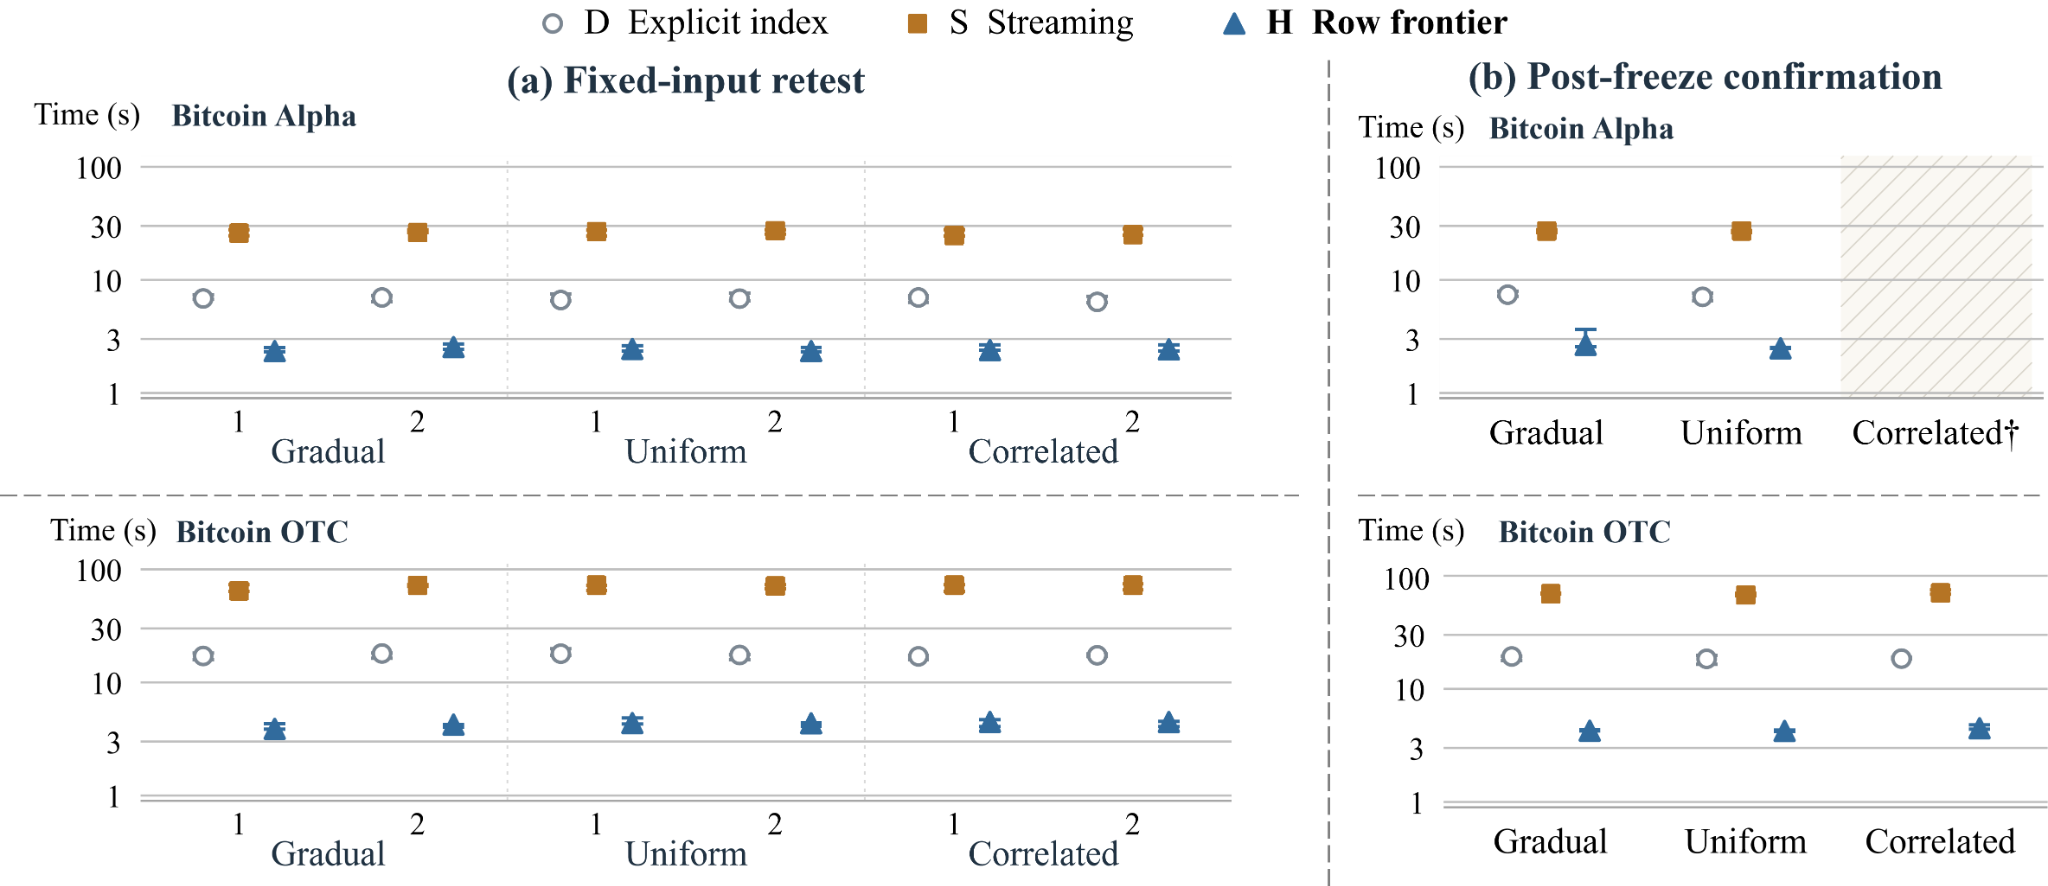
\includegraphics[width=\textwidth]{user_originals/fig2.png}
\caption{Complete setup-plus-Q4 costs of explicit indexing (D), streaming (S), and row-frontier access (H) under the original instrumented policy. (a) Twelve previously diagnosed streams, with labels 1 and 2 identifying two inputs per graph and opinion family. (b) Six streams generated after implementation freezing. Gradual, uniform, and correlated denote gradual-change, independent-uniform, and signed-neighbor opinions. Markers show medians; whiskers span three-repeat minima and maxima on logarithmic time axes. The hatched $\dagger$ cell has no complete Q4 time (Section~\ref{sec:completion}).}
\Description{Two rows show Bitcoin Alpha and OTC. The fixed-input retest appears on the left and post-freeze confirmation on the right. H has lower complete costs than D and S on the completed streams. The Alpha correlated confirmation cell is hatched and marked with a dagger because no complete Q4 timing is available.}
\label{fig:costs}
\end{figure*}

% P:HG1
\textbf{The alternative cover lowers complete cost.} Under common \texttt{light\_v1} measurement on the same five completed streams, G uses 12.56\% less aggregate service time than H: 18.833572 versus 21.537746 seconds over 15 pairs. G is faster in 14 pairs, and all five per-stream median ratios favor G (Figure~\ref{fig:hg_costs}). The following work analysis explains how cheaper coverage preparation offsets greater response demand.

\begin{figure}[t]
\centering
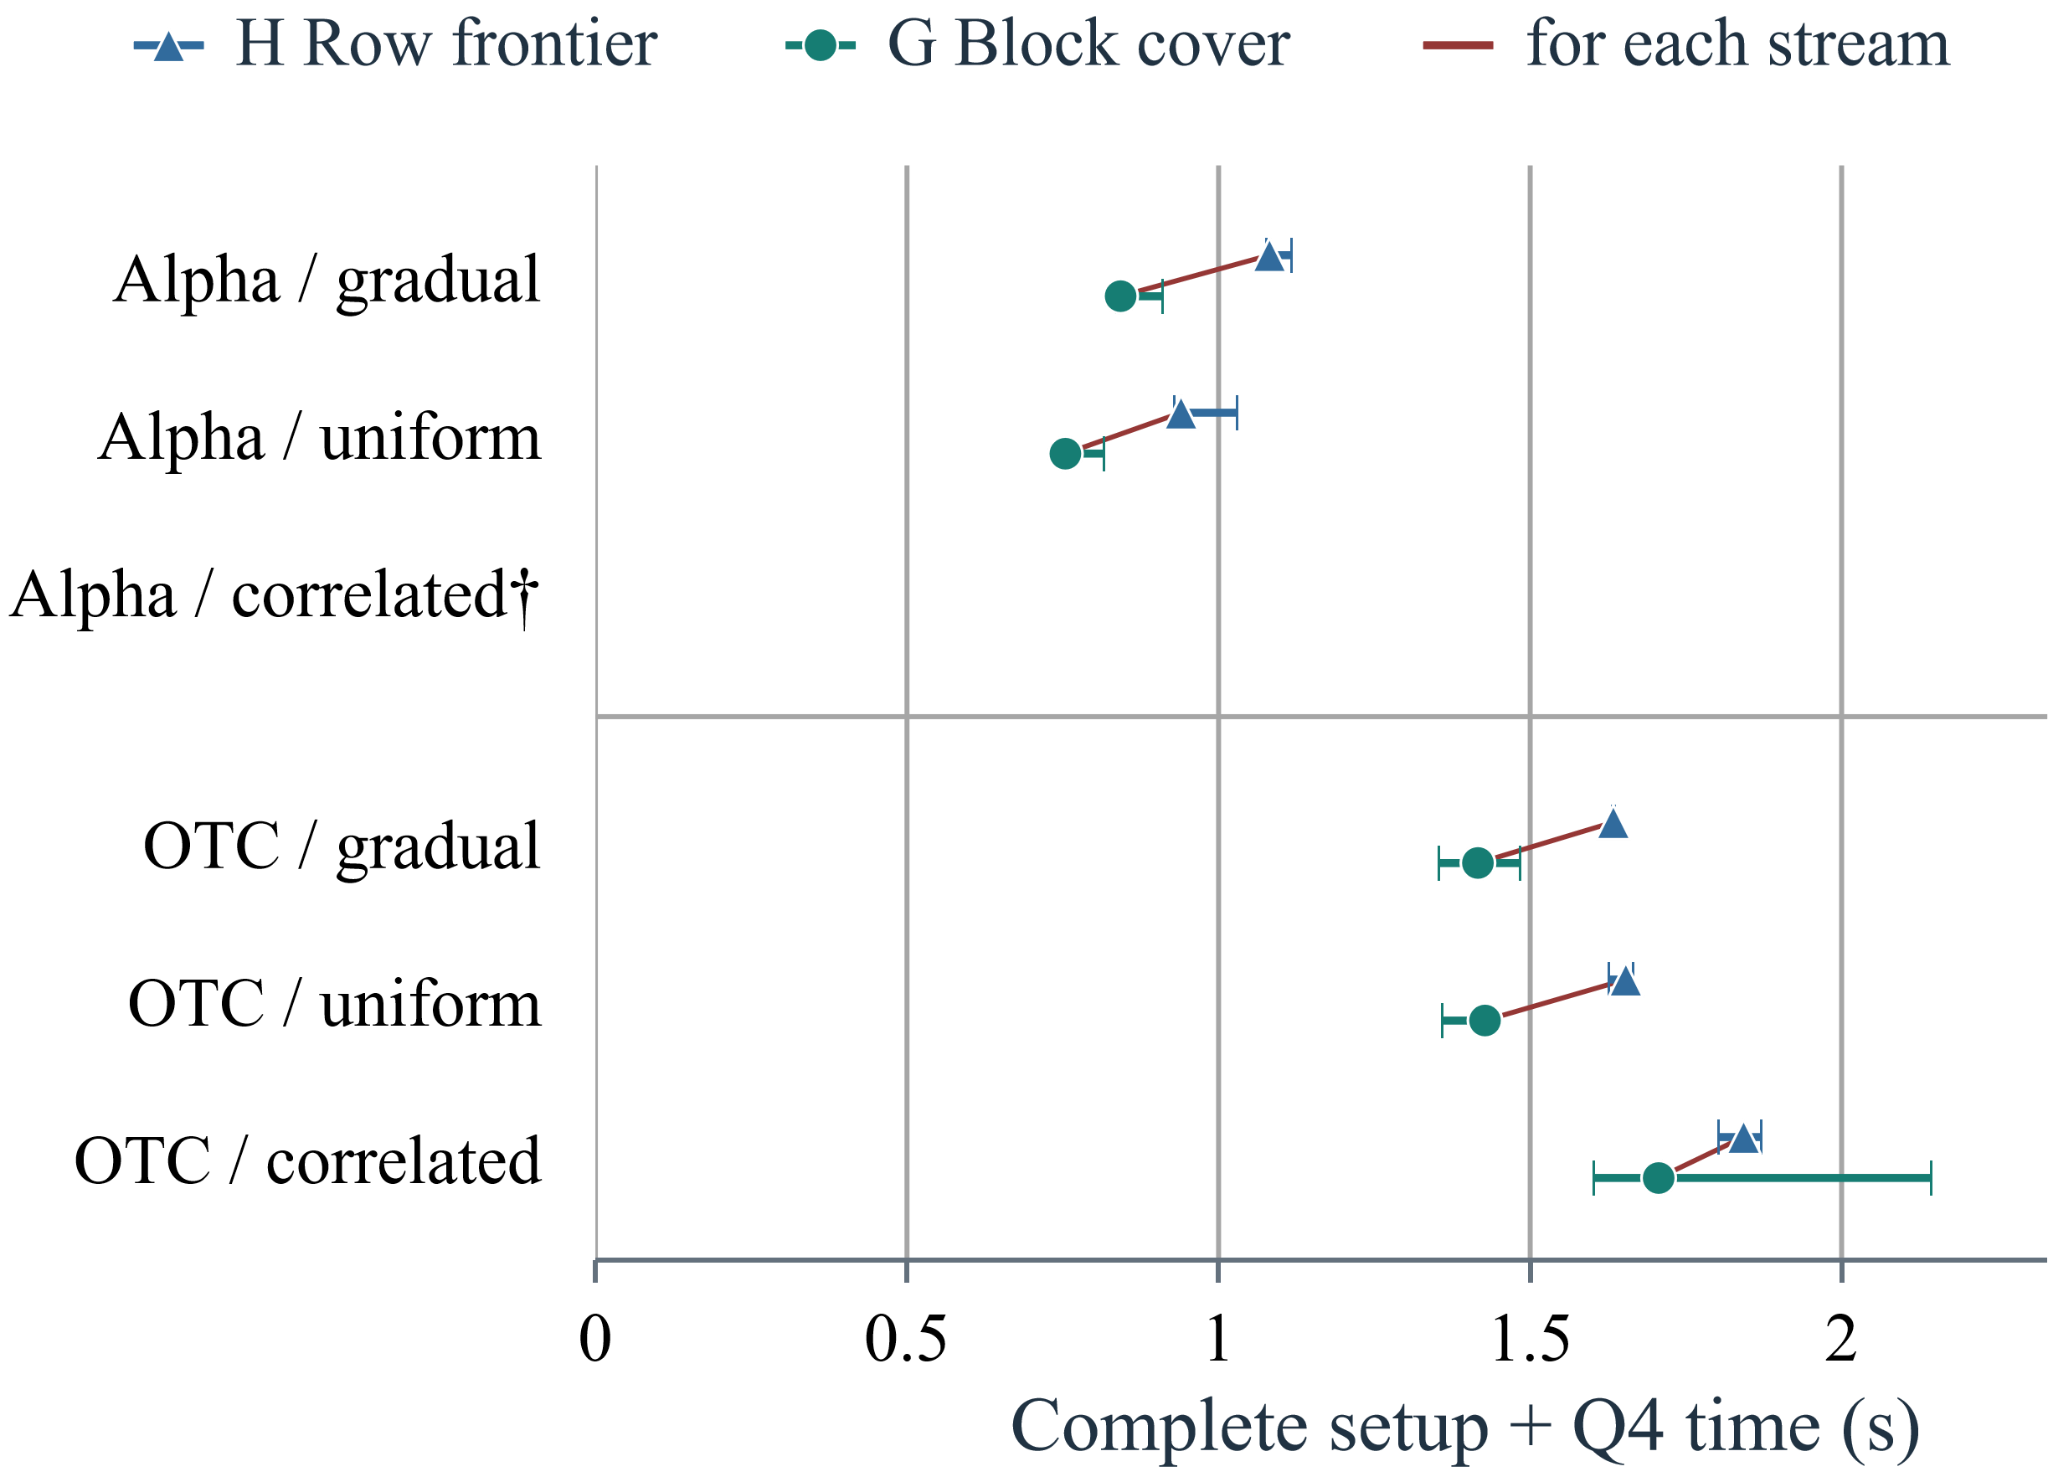
\includegraphics[width=\columnwidth]{user_originals/fig3.png}
\caption{Complete setup-plus-Q4 costs of row-frontier access (H) and block coverage (G) under common \texttt{light\_v1} measurement on the same six confirmation streams. Markers show medians; whiskers span the minimum and maximum of three timing repeats. Red segments connect H/G medians for the same stream. Opinion labels follow Figure~\ref{fig:costs}. $\dagger$ marks Alpha/correlated, for which no complete Q4 cost is available (Section~\ref{sec:completion}).}
\Description{Horizontal timing ranges compare H and G on Alpha and OTC. Blue triangles and green circles show method medians, and red segments join medians for each stream. G has a lower median in all five completed streams. The Alpha correlated stream remains as a dagger-marked row with no complete timing.}
\label{fig:hg_costs}
\end{figure}



\subsection{RQ2: Where Does Coverage Save Work?}
% P:E7
The diagnosed retest exposes an access-work difference with matching response demand: H and D have equal graph-level mean Gram and response-block counts, while D processes about 470 and 784 times as many endpoint rows on Alpha and OTC. H pays for all 60 frontier builds per completed Q4. Median peak RSS over 18 workers per graph and method is 108.45/124.76 MiB for H, versus 583.19/1,216.81 for D. Streaming uses similarly low memory to H but scans hundreds of millions to over a billion endpoint rows per Q4. Implicit representation and selective access thus address different costs. RSS includes factors, caches, and runtime objects.

% P:E8
G shifts work from coverage preparation to numerical response acquisition. Over the same 15 complete H/G pairs, it sends fewer cold rows to endpoint screening and requests more RHS columns, scores, Grams, and transfers (Table~\ref{tab:hg_work}). Cold rows count inputs to endpoint screening. Mutually exclusive phase totals for H/G are 5.936/2.258 seconds in frontier preparation, 5.582/6.115 in response acquisition, and 0.868/0.934 in transfer. The reduction in preparation cost more than offsets the additional numerical work, explaining G's lower complete-service time on these inputs.

\begin{table}[t]
\centering
\caption{Work over the 15 complete H/G pairs under \texttt{light\_v1}: 60 requests and 900 accepted records per method.}
\label{tab:hg_work}
\begin{tabular}{@{}lrr@{}}
\toprule
Recorded work & H & G\\
\midrule
Cold rows sent to screening & 6,081 & 741\\
Candidate RHS columns & 2,214 & 2,277\\
Worker scalar RHS (all roles) & 3,081 & 3,150\\
Scoring calls & 3,789 & 4,056\\
Gram materializations & 1,305 & 1,320\\
Transfer items & 3,540 & 3,777\\
\bottomrule
\end{tabular}
\end{table}

% P:E8a
The mechanism records show how G obtains its coverage. Collapsing timing repeats by graph, root, catalog, opinion, and parent identity yields 300 decision states in the completed streams. G excludes the entire insertion class in 44\% of these states and enters block access in the remaining 56\% (Table~\ref{tab:g_mechanism}). Insertions win 34\% of decisions; moreover, 66 of the 198 flip winners also enter block access. Both whole-class exclusion and block search therefore participate in the measured execution. The artifact retains the corresponding counts for all six streams.

\begin{table}[t]
\centering
\caption{G mechanisms in five complete streams: 300 distinct decision states after removing timing repetitions. The two pairs of rows are separate partitions of the same states.}
\label{tab:g_mechanism}
\begin{tabular}{@{}lrr@{}}
\toprule
Observed property & States & Share\\
\midrule
Whole insertion class excluded & 132 & 44\%\\
Block access entered & 168 & 56\%\\
\midrule
Flip selected & 198 & 66\%\\
Insertion selected & 102 & 34\%\\
\bottomrule
\end{tabular}
\end{table}

% P:S1
\textbf{Catalog storage and numerical preparation.} A startup test on Slashdot, with $82{,}140$ vertices, separates these two costs~\cite{snapslashdot,leskovec2010signed}. D's required explicit payload is estimated at 53.404 GiB, so the 4-GiB address-space preflight prevents startup. H and S avoid that allocation; their shared SuperLU root preparation reaches the 600-second limit before the first request. This test identifies numerical preparation as the remaining startup barrier; stage and memory records are in the artifact.



\subsection{RQ3: What Do Response Maintenance and Directional Bounds Save?}
% P:E9
To examine response maintenance separately from all-nonedge access, a fixed-catalog study uses supplied catalogs of 1,000/2,500 candidates and budgets of 20/40. Its six graphs are unit-signed Alpha, OTC, and Slashdot plus controlled Conflict, Bio, and Fin graphs; $\alpha=1$, edit weights are one, opinions are bounded, and $\delta=10^{-9}$. Ten isolated single-threaded repetitions on an Intel Core i7-12700H under Windows compare Jacobi-preconditioned conjugate gradient (CG) and the CHOLMOD sparse Cholesky backend~\cite{chen2008cholmod,virtanen2020scipy}. Within each backend, cold solves, within-version caching, and planned transfer share the trajectory. Each comparison pairs policies within the same backend and environment.

% P:E10
In the six-graph, 2,500-candidate, 40-commit slice, planned CG and CHOLMOD use 1,393 and 1,407 scalar response RHS columns, including winner and refresh work, versus 15,054 for cold CG. Initialization-inclusive median times on Alpha decrease from 6.29 to 0.984 seconds for CG and from 1.08 to 0.424 for CHOLMOD; on OTC they decrease from 12.4 to 1.44 and from 2.34 to 0.613. These matched-backend comparisons support maintaining requested responses in this fixed-catalog setting. The complete six-graph table remains in the artifact.

% P:E11
The directional study asks whether bounding the queried direction reduces uncertainty on the same approximate inputs. It uses 60 negative Alpha hub edges and 72 disjoint negative Bio edges at weights $1,4,16,64$. Eight settings and 20 initial-tolerance runs yield 41,744 paired events before additional refinement or reanchoring; accepted rounds include every remaining candidate, and stop rounds add no events. Table~\ref{tab:directional}'s \emph{same-state} column compares raw normwise and directional radii on identical stored states, responses, and error histories, each with its own center. Its \emph{policy-history} column compares executions at the same candidate/version whose maintained errors and reanchor histories may differ.

\begin{table}[t]
\centering
\caption{Directional stress: median ratios of recorded normwise to directional radii. Same-state pairs share approximate inputs and error histories; policy-history pairs match the candidate and version. Each row includes all recorded tolerances and events.}
\label{tab:directional}
\begin{tabular}{lrrrr}
\toprule
Graph & Weight & Events & Same state & Policy history\\
\midrule
Alpha & 1 & 1,010 & 2.94 & 2.94\\
      & 4 & 1,010 & 8.47 & 8.67\\
      & 16 & 840 & 32.12 & 47.86\\
      & 64 & 884 & 140.49 & 757.44\\
Bio   & 1 & 9,500 & 5.17 & 5.24\\
      & 4 & 9,500 & 35.82 & 38.11\\
      & 16 & 9,500 & 669.49 & 528.49\\
      & 64 & 9,500 & 32,678.41 & 7,809.73\\
\bottomrule
\end{tabular}
\end{table}

% P:E12
Directional radii are smaller in all 41,744 paired events, with the largest median reductions at high weights. In the Bio policy comparison at weight 64, budget 50, and initial CG tolerance $10^{-5}$, reanchors decrease from 2,375 to 59 and response blocks from 2,496 to 180. This connects tighter enclosures to less response maintenance on that workload. These results compare archived radius and maintenance records; the artifact documents their audit scope.

\subsection{RQ4: Which Decisions Are Independently Verified?}
\label{sec:completion}
% P:E13
The checker asks whether a reported winner has positive gain and satisfies the current comparison against every legal rival. It reconstructs the root, exact opinion, catalog, chosen set, and selected children, independently of the execution frontier. Small graphs permit exact rational evaluation. On larger graphs, any trial $x\in\R^n$ gives
\begin{equation}
 2s^\top x-x^\top Ax\le s^\top A^{-1}s
 \le2s^\top x-x^\top Ax+\|s-Ax\|_2^2.
 \label{eq:checker-energy}
\end{equation}
The difference from the lower expression is $(s-Ax)^\top A^{-1}(s-Ax)$, bounded by the squared residual since $A\succeq I$. Dyadic integer arithmetic evaluates the enclosure; CG supplies only a trial. The checker enumerates every legal pair in bounded blocks, using its own endpoint caps and child-energy bounds, and records counts and a digest of the identifier stream.

% P:E15
The checker certifies winner positivity and all-rival comparison using its own evidence, and verifies online equality witnesses through parent and opinion invariance and child conjugacy. It separately checks published intervals: containment of the exact gain on rational instances, and nonempty intersection with an independent enclosure on larger instances. The latter is an interval-consistency check; the final decision is verified with the independent bounds.

% P:E18
All 30 decisions in two preselected H requests pass independent full-catalog replay. The requests are q1 of the independent-uniform stream on each graph, using V2 repetition zero. Table~\ref{tab:verification} places these results alongside fixed-input replays and structural or record-based checks. Checker time is accounted for separately from service cost.

\begin{table}[t]
\centering
\caption{Independent replay and complementary checks. Exec. counts request executions. The G row links 90 observations to the same 30 states replayed for H; verification populations can overlap.}
\label{tab:verification}
\begin{tabularx}{\columnwidth}{lrrY}
\toprule
Check & Exec. & Records & Scope\\
\midrule
Diagnosed fixed inputs & 10 & 150 & Full-domain replay\\
Fixed timed OTC & 1 & 15 & Full-domain replay\\
Fixed timed chains & 432 & 6,480 & Bindings and structural equality\\
V2 preselected H & 2 & 30 & Full-domain replay\\
V4 request records & 144 & 2,088 & Recorded agreement\\
G archive-derived & 6 & 90 & Interval containment\\
\bottomrule
\end{tabularx}
\end{table}

% P:E18a
\textbf{Linking the replay to G.} The same 30 replayed states support a derived check of G's published gains. Original inputs and recorded chains bind the graph, opinion, parent state, legal domain, and winner. Across three G repeats, all 90 observations satisfy $I_{\rm independent}\subseteq I_G$: the published interval contains the archived independent enclosure. This checks G's outputs at matched states, rather than independently replaying its block-pruning decisions.

% P:E19
\textbf{A structural explanation for the Alpha overlap.} An offline witness combines two vertex swaps that preserve the current parent and opinion and map the two specified children, proving equal gains. This establishes the candidate pair's exact equality. The online resolver supports single-swap witnesses, so the complete decision remains unresolved after three accepted edits. The artifact records the permutation and its bindings.
